%%%%%%%%%%%%%%%%%  Debut du fichier Latex  %%%%%%%%%%%%%%%%%%%%%%%%%%%%%%
\documentclass[
    a4paper, 
    12pt, onecolumn,
    %draft
]{article}

%%% Pour un texte en francais
\usepackage{cite}
\usepackage{amssymb, amsmath}
\usepackage{lineno}

\usepackage {dsfont}
%\usepackage[ruled,vlined, linesnumbered]{algorithm2e}
\usepackage{algorithmic}
\usepackage{algorithm}
\usepackage{math}
\usepackage{float}
\usepackage{times}
\usepackage{amssymb}
\usepackage{amsfonts}
\usepackage{slashbox}
\usepackage{makeidx}
\usepackage{color}


%\usepackage[francais]{babel}
%\usepackage[latin1]{inputenc}	         % encodage des lettres accentuees
\usepackage{graphicx} \def\BIB{}
\usepackage{url}

\usepackage[textwidth=17mm]{todonotes}
\newcommand{\customtodo}[4]{
        \todo[color=#2,inline,size=\small]{
                \ifx&#3&
                        \textbf{#1} #4
                \else
                        \textbf{#1$\Rightarrow$#3} #4
                \fi
        }
}
\newcommand{\HC}[2][]{\customtodo{HC}{red!20}{#1}{#2}}
\newcommand{\IF}[2][]{\customtodo{IF}{blue!20}{#1}{#2}}

\newcommand{\ie}[0]{{\em i.e.},\xspace}
\newcommand{\vs}[0]{{\em vs.}\xspace}
\newcommand{\eg}[0]{{\em e.g.},\xspace}
\newcommand{\etal}[0]{{\em et al.}\xspace}
\newcommand{\wrt}[0]{{\em w.r.t.}\xspace}
\newcommand{\aka}[0]{{\em a.k.a.}\xspace}
\newcommand{\via}[0]{{\em via}\xspace}

%--------------------------------------------------------

\title{Fog-RAN placement problem}
\author{Hélène Coullon (Inria, IMT) and Ilhem Fajjari (Orange Labs)}

\begin{document}

\maketitle

%---------------------------------------------------------
\section{From RAN to Cloud-RAN to Fog-RAN}
%---------------------------------------------------------
\IF{Ilhem, add your comments by using this command}
\HC{Helene, add your comments by using this command}

\IF{Introduction}
\textcolor{blue}{
Mobile broadband services services have notably proliferated over the last few years leading to the explosion of the number of smart devices which has grown into billions. Next-generation Radio Access Networks (RANs) are expected to support 1000-fold more traffic and 10-fold lower latency while minimizing the cost and energy consumption of network deployment~\cite{CITE-001}. Some envisioned solutions consist in extending the network by a dense deployment of cells building a Heterogeneous Network (HetNet)~\cite{CITE-002} and using additional spectral resources with more advanced techniques for interference management like the enhanced Inter Cell Interference Control (eICIC)~\cite{CITE-003}. However, deploying such solutions in the existing architecture would require high CAPpital EXpenditure (CAPEX) and OPerational EXpenditure (OPEX) and  will inevitabley lead to  bandwidth bottleneck between distributed base stations~\cite{CITE-004}.
}


\textcolor{blue}{
To overcome this issue, Cloud RAN architecture (CRAN)~\cite{CITE-005} has been proposed to adopt the cloud computing concept for future cellular networks by decoupling the traditional eNodeB into baseband unit (BBU) centralized in the cloud and a remote radio unit (RRU) remaining at the access site with a network interconnecting the central site to the access sites termed as fronthaul. Such a centralized architecture comes from pooling the BBUs of multiple cells and deploying them in a cloud environment with commodity hardware and virtualization techniques which offer statistical multiplexing gains of resources and energy efficiency~\cite{CITE-006}. Additionally, the CRAN concept takes benefits from collocated BBU processing facilitating more the Coordinated Multi-Point processing (CoMP) which requires stringent synchronization constraints between cells being hardly satisfied in current distributed architecture~\cite{CITE-007}
}

A Radio Access Network (RAN) is a part of a mobile telecommunication system. RAN resides between a mobile device (such as mobile phones or tablets) and the core network (CN)~\footnote{\url{https://en.wikipedia.org/wiki/Radio_access_network}}.

Distributed RAN~\footnote{\url{https://en.wikipedia.org/wiki/C-RAN}} architecture has been introduced for the 3G technology. Unless 1G and 2G architectures, where base stations were responsible for all signal computations, for 3G a distributed base station architecture has been introduced by Nokia, Huawei etc. In this architecture the radio function unit, or Remote Radio Head (RRH) is separated from the baseband unit (or BBU) by a fronthaul network (fiber), which results in lighter base stations that can be placed directly close to antennas, thus reducing signal loss.

The major difficulty of this system is to perfectly choose the size of BBUs pool. In pratice, these pools are designed to answer a very high load onto the network which results in an under-use of the pool most of the time, thus non optimized costs.

To optimize BBUs usage, the Cloud-RAN~\footnote{\url{https://en.wikipedia.org/wiki/C-RAN}} architecture has been proposed. In this solution BBUs become BBUs-as-a-Service accessible into a centralized private or public Cloud, on demand, thus increasing flexibility and elasticity of the architecture and reducing costs.

However, latencies to the Cloud could be too high to reach high speed mobile network such as 4G and 5G. Actually, BBUs are responsible for all L1/L2/L3 functions of the OSI standard. Some of those functions, for example the ones of the physical layer, require a low response latency of 1 to 5 milliseconds.  For 5G, latencies constraints could even need a heart beat in micro seconds. Moreover the physical layer also requires a strong synchronization of information with RRHs resulting in bandwidth issues when BBUs are placed in a centralized Cloud.

For this reason, new generation of distributed Clouds such as Fog computing are studied for RAN. In Fog computing core network (CN) devices, such as routers, which are placed at key point of the network are used to deploy micro data centers. As a result, the number of hops between clients and data centers are reduced, the load per micro data centers is reduced, the energy consumption as well as security policies of data centers are easier to control.

\textcolor{blue}{
In order to relax these stringent fronthaul constraints and  hence take advantage of  the baseband unit centralization,  both industrial and academic institutions are rethinking the CRAN architecture to hybrid solution that places the BBU functionalities in a flexible way between the central site and the traditional access site, both connected through a so called fronthaul link~\cite{CITE-012, CITE-013, CITE-014, CITE-015,  CITE-028}. Accordingly, many possible interfaces between BBU functions are being identified referring to the traditional LTE architecture so-called as functional splits~\cite{CITE-017} in a way that some of the resulting BBU processing sub-functions can be gradually migrated to the access site for less barden on the fronthaul link at the expense of loosing some gain from BBU centralization~\cite{CITE-018}.
}

%---------------------------------------------------------
\section{Infrastructure}
%---------------------------------------------------------
The overall infrastructure is composed of
\begin{itemize}
\item N base stations;
\item A fronthaul network;
\item A fog infrastructure;
\end{itemize}
as represented in Figure~\ref{fig:infra}.

Each base station is defined as a node with associated CPU, RAM and DISK capacities. In this work we consider a single base station which is the source of the demand. The fronthaul network is associated to a bandwidth and a latency. One can note that the latency of a network connection can increase depending on the charge of the link, thus the indicated latency is the best possible latency on the link.

The fog infrastructure is represented as a graph $G(V,E)$, where
\begin{itemize}
\item V is the set of nodes or servers, each one associated to the triplet $(CPU,RAM,DISK)$ capacities
\item E is the set of network links between two nodes, each one associated to the pair $(bandwidth,latency)$
\end{itemize}

\begin{figure}[t]
\begin{center}
  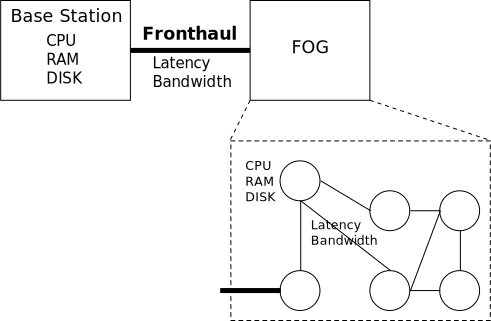
\includegraphics[width=.7\textwidth]{./images/infra.pdf}
  \caption{Fog-RAN infrastructure}
  \label{fig:infra}
\end{center}
\end{figure}

%---------------------------------------------------------
\section{Placement Problem}
%---------------------------------------------------------
A research difficulty associated to the Fog-RAN vision is where to place network functions of the BBU onto the distributed infrastructure such that functions requirements regarding CPU, RAM, latency etc. are respected and such that the overall cost is minimized. Current Cloud-RAN solutions place all BBUs functions onto the centralized Cloud.

%---------------------------------------------------------
\subsection{Split-based Placement Problem} \IF{This section is reformulated}
%---------------------------------------------------------
The first solution is based on 7 possible splits of BBU functions. BBU functions are organized into seven different categories: RF, L1-low, L1-high, L2-low, L2-high, L3-low, L3-high. A split is composed of two sides, one side will be placed onto the RRH, the other side will be placed onto one server of the Fog infrastructure.

The seven possible splits are:
\begin{itemize}
\item RRH: RF - BBU: L1/L2/L3
\item RRH: RF/L1-low - BBU: L1-high/L2/L3
\item RRH: RF/L1 - BBU: L2/L3
\item RRH: RF/L1/L2-low - BBU: L2-high/L3
\item RRH: RF/L1/L2 - BBU: L3
\item RRH: RF/L1/L2/L3-low - BBU: L3-high
\item RRH: RF/L1/L2/L3 - BBU: nil
\end{itemize}

% constraints
Considering a given source (base station), the placement problem is to choose the best split and the best server on which to place BBU functions. This placement problem should take into account the following constraints:
\begin{itemize}
\item answer CPU needs for functions placed onto a Fog server;
\item answer latency constraint between functions placed at RRH and functions placed in the Fog according to the fronthaul and CN network;
\item answer the required bandwidth.
\end{itemize}

% algorithm
The algorithm could be the following
\begin{enumerate}
\item input: demand
\item compute the 7 possible splits of the demand with associated constraints (CPU, latencies, bwdth)
\item for each split solve a placement problem to select the best server on the Fog infrastructure
\item apply a final objective function to select the best solution among the seventh best solution (one for each split)
\end{enumerate}

Definition of the placement problem (3):


\begin{figure}[t]
\begin{center}
  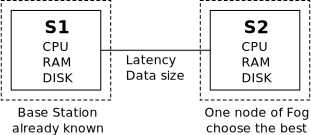
\includegraphics[width=.55\textwidth]{./images/app1.pdf}
  \caption{Split-based Fog-RAN}
  \label{fig:app1}
\end{center}
\end{figure}

\IF{Hereafter the new section}

\subsection{Functional Split Model}
\textcolor{blue}{
We model the baseband processing of one cell as a chain of processing functions (PFs) includng $K_{cell}$ Cell-Processing (CP) functions and $K_{user}$ User-Processing (UP) functions as shown in Fig.~\ref{fig:2} where we can find:
\begin{itemize} 
\item PF1 which conducts the platform control proccessing with Medium Access Control (MAC), Radio Link Control (RLC) and Packet Data Convergence Protocol (PDCP),
\item PF2 is per-user basis performing turbo encoding, forward error correction (FEC) and rate matching,
\item PF3 is per-user basis and includes quadrature amplitude modulation (QAM) that generates symbols for multi-antenna mapping,
\item PF4 starts the cell processing by mapping the symbols on resource elements,
\item PF5 adds the cyclic prefix and transforms symbols from frequency domain to time domain using Fast Fourier Transform Algorithm,
\item PF6 generates the RF signals and conducts the parallel-to-serial conversion among others. 
\end{itemize} 
}
\vspace{0mm}
\begin{figure}[t!]
\begin{center}
\begin{tabular}{c}
\hspace{-0mm}
\includegraphics[scale=0.3]{./images/splits.png}
\end{tabular}
\end{center}
\vspace{-3mm}
\caption{\label{fig:2} Functional Splits}
\end{figure} 
\textcolor{blue}{
In order to quantitatively study the computational cost of functional splits, we refer to the conducted analysis by~\cite{CITE-020} where the amount of computational resources is expressed in Giga Operations Per Second (GOPS) and calculated as the PF’s reference GOPS value multiplied by a scaling function of configuration parameters which include the carrier bandwidth (B), number of antennas (A) and user traffic load (B)~\cite{CITE-020}. As PF5 and PF6 are cell processing for time-domain and PF1 is platform control proccessing, their computational requirement is load independant. PF2, PF3 and PF4 are processing in frequency domain so they take into account only frequency carriers having data signals which make them load dependant.
}
\begin{equation*}
\begin{aligned}
&PF_{1} : g_1 = G_{1}^{ref} . \frac{A}{A_{ref}} \\
&PF_{2} : g_2(M_i,L_i) = G_{2}^{ref} . \frac{B }{B_{ref}} .  \frac{M_i }{M_{ref}} . \frac{A}{A_{ref}} . \frac{L_i}{L_{ref}} \\
&PF_{3} : g_3(L_i) = G_{3}^{ref} . \frac{B }{B_{ref}} . (\frac{A}{A_{ref}} )^2 . \frac{L_i}{L_{ref}} \\
&PF_{4} : g_4(L[]) = G_{4}^{ref} . \frac{B }{B_{ref}} . \frac{A}{A_{ref}} . \sum_{i}^{Users}  \frac{L_i}{L_{ref}} \\
&PF_{5} : g_5 = G_{5}^{ref} . \frac{B }{B_{ref}} . \frac{A}{A_{ref}} \\
&PF_{6} : g_6 = G_{6}^{ref} . \frac{B }{B_{ref}} . \frac{A}{A_{ref}} \\
\end{aligned}
\end{equation*} 
\textcolor{blue}{
In the same way, we refer to the work of~\cite{CITE-008} to quantify the impact of functional split on the generated rate on the fronthaul link. According to this model, the estimated bandwidth between BBU functions is calculated as a function of number of antennas (A) and user traffic Load (B).  
}
\begin{equation*}
\begin{aligned}
&Split_D  : f_0(L[]) = \alpha_0 . \sum_{i}^{Users} L_i\\
&Split_{1}  : f_1(L_i) = \alpha_1 . L_i\\
&Split_{2}  : f_2(M_i,L_i) = \alpha_2(M_i) . n_{RB} . L_i + \beta_1 \\
&Split_{3}  : f_3(L_i) = \alpha_3 . A . n_{RB} . L_i + \beta_2 . A\\
&Split_{4}  : f_4 = \alpha_4 . A. n_{RB} \\
&Split_{5}  : f_5 = \alpha_5 . A . n_s \\
&Split_C  : f_6 = \alpha_6 . A . n_s 
\end{aligned}
\end{equation*} 
\textcolor{blue}{
By considering the downlink transmission direction, user processing functions (PF1, PF2 and PF3) are generating data rate that scales with user load making the fronthaul link corresponding to split $0$, split $1$, split $2$ and split $3$ load dependant. Cell processing functions are a sequence of functions in the physical layer where UEs signals are multiplexed which makes the computational requirement load independant generating constant traffic rate for any amount of cell load. With considering the latency requirements~\cite{CITE-008}, once the HARQ process located in MAC layer is placed in the edge site, latency requirement is significantly relaxed.
}
%---------------------------------------------------------
\subsection{Function-based Placement Problem} 
%---------------------------------------------------------
The other solution is to not limit the placement to only two sides (i.e., RRH and BBUs) but to consider each function to place separately, which is closer to a usual placement problem.

In this case you will have to consider two input graphs. The first one represents the infrastructure topology (like in the first case), with nodes representing servers and links representing networks. The second one represent the graph of dependencies between BBUs functions and their associated CPU, latencies and bandwidth requirements.

\begin{figure}[t]
\begin{center}
  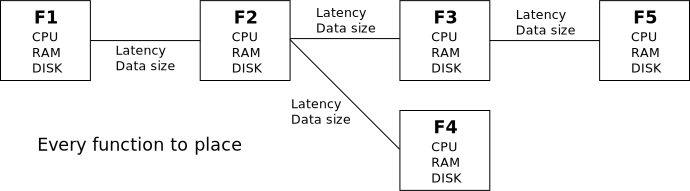
\includegraphics[width=\textwidth]{./images/app2.pdf}
  \caption{Function-based Fog-RAN}
  \label{fig:app2}
\end{center}
\end{figure}

%---------------------------------------------------------
\section{Related Work}
%---------------------------------------------------------
\IF{added SoA} 
\textcolor{blue}{
Currently, research perspective looks for finding intermediate RAN architectures between the Centralized RAN and the Distributed RAN by identifying the possible levels at which the traditional eNodeB functions should be splitted. Each option is analyzed to identify the requirements in terms of resource capacities and latency~\cite{CITE-015, CITE-017, CITE-021}. Next Generation Mobile Networks (NGMN) alliance highlighted in~\cite{CITE-014} the need for a splitted RAN architecture and studied different splits in uplink and downlink. Next Generation Fronthaul Interface (NGFI) has proposed in~\cite{CITE-021} an Ethernet-based Next Generation Fronthaul Interface architecture with different functional splits between RRU and the Radio Cloud Center(RCC) having a fronthaul architecture with link aggregators termed as Radio Aggregation Units (RAU). 3GPP supports functional splits in~\cite{CITE-023} to add more flexibility to hardware implementation and build scalable cost effective solutions. It also brings the possibility for load management, optimisation and network slicing operation~\cite{CITE-024}. Small cell forum (SCF) analyzes in~\cite{CITE-015} different splits (PDCP/RLC/MAC/PHY) for a small cell but also “fractional splits” that corresponds to split-MAC and split-PHY. They introduces a split between the RRC and PDCP layers offering the possibility to separate the control and data-planes.
}
\textcolor{blue}{
Based on these perspectives, there is a strong interest from telecom industry to leverage BBU functional split in providing a cost-effective transport network. Authors of~\cite{CITE-025} build a graph based framework to reduce the total cost of computational and fronthaul by optimally placing  the BBU functions between clusters representing central and access sites. ~\cite{CITE-026} proposes a total cost of ownership (TCO) minimization model with different functional split decision options taking into account base station configuration and data transmission direction. Authors in~\cite{CITE-027} evaluate the impact of different transport protocols on different split levels and propose a framework architecture for dynamic functional split deployment to meet the bandwidth and delay requirements in a real time. Fronthaul link performance is evaluated in~\cite{CITE-011} for different packetization strategies. In~\cite{CITE-018} teletraffic theory is adopted to analyze the fronthaul for statistical multiplexing gain in a hybrid RAN and the impact of function splits on the energy and cost savings. Nevertheless, the above methods propose a splitted fronthaul per cell and do not consider traffic heterogeneity, and hence, seen as a monolithic and not flexible architecture serving all type of end users. The authors of ~\cite{CITE-028} propose a model that aims to minimize the system energy and bandwidth consumption on fronthaul by adopting user functional splits but still does not consider the heterogeneity of user service requirements and does not analyze the impact of user load on split decisions.
}


Paper~\cite{7371709} presents NACER, a network-aware cost efficient resource allocation method for
processing-intensive tasks in distributed Clouds. In the context of a distributed small DCs, this paper modelized a placement problem to answer VM requirements while minimizing inter-DCs communication costs. An advanced greedy algorithm is build by using the A* search algrotihm borrowed from Artificial Intelligence. Results are simulated inside CloudSIM and show very interesting results compared to simple greedy and random algorithms. It also offers an interesting state of the art analysis of other papers already read~\cite{Alicherry2012NetworkAR,6566850,7872914}. Most of them are using greedy algorithms.

None of the read paper address latencies as a strict constraint to respect~\cite{Alicherry2012NetworkAR,6566850,5662521,Steiner:2012:NSP:2377677.2377687,5461930,7872914}. All of them study the minimization of the communication cost (which is non linear and NP-hard). Handled constraints respect processing or memory requirements (linear formulation).

\cite{6217419} present a SLA-based optimization of Power and Migration Cost in Cloud Computing. The interesting part of the paper concerning our work is the model of performances, which is directly linked to latencies and response time. the response time follow an exponential distribution and time response are guaranteed in most cases with an additional penalty cost when the latency is exceeded.

\cite{silvaeuropar} present a very interesting work that takes into account latency constraints. The work modelise the network topology and the component-based application by adding a connection quality concept that reflects latencies. The network topology is modelized as a tree where leaves represents VM types or physical machines, and where inner nodes represents connections between leaves at different levels of the tree. The number of inner nodes (hops) to pass to communicate with another VM or machine thus represents the connection quality or latency. On the other hand the same connection quality is used to indicate required communication quality expected between two components of the application. Authors both consider usual bin-packing problem (requirements on capacities and cost minimization) while also taking into account communication constraints. The presented heuristics is based on a divide-and-conquer mechanism to be scalable. It first decompose the problem into sub-problems and then compose solutions to build the final placement. Papers cited that have to be read are~\cite{6253484,6256562,6495451,5461930}.

to read~\cite{Meng:2010:ERP:1809049.1809052}

%---------------------------------------------------------
\section{Discussion}
%---------------------------------------------------------
\paragraph{Split Constraints.} As BBUs functions are very well known, mathematical models exists to determine, from a given split, the expected latency between the two sides of the split, as well as CPU and RAM needed for the set of BBU functions placed onto a cloud infrastructure.
\HC{Ilhem j'aimerais avoir des détails sur ces modeles}
\IF{J'ai rajouté les modèles dans la section problem}

\paragraph{Latency Constraints} Guaranteeing a latency is very difficult as it is traffic-dependent. Latencies can be more or less predicted if the network-usage is perfectly known and controlled, however, in such case the network is private and the elasticity is reduced (as in HPC clusters, private Clouds or private servers). Static models can be defined but they will not reflect reality but an approximation of the reality like in~\cite{silvaeuropar}. Dynamic models would probably be more realistic but costly (migrations, computations on the fly etc.). Another possibility is to approximate the reality but to introduce penalties when latencies are not respected. In such case, answering expected latencies is not guaranteed, as a constraint, but is included into cost minimization objectives.


\bibliographystyle{plain}
\bibliography{fogran}



\end{document}



